\documentclass{article}  
\usepackage{graphicx}
\usepackage[utf8]{inputenc}
\usepackage[T1]{fontenc}
\usepackage{float}
\usepackage[italian]{babel}
\usepackage{listings}
\usepackage[usenames]{color}
\usepackage{natbib}
\usepackage{siunitx}
\usepackage[strict]{changepage}
\usepackage{physics}
\usepackage{wrapfig}
\usepackage[a4paper, top=2cm, bottom=2cm, right=2cm, left=2cm]{geometry}
\usepackage{array}
\usepackage{color}
\usepackage{colortbl}
\usepackage{amsmath}
\usepackage{amssymb}
\usepackage{multirow}
\usepackage{enumitem}
\usepackage{hyperref}
\usepackage{times}
\usepackage{booktabs}
\usepackage{subfig}
\usepackage{multirow}



\title{Effetto Zeeman}
\author{Docente: dott. Garfagnini, dott. Lunardon \\
Gruppo 14}
\date{Anno accademico 2019/20}

\begin{document}



\maketitle

    \begin{itemize}
        \item[$\circ$] Aidin Attar - 1170698 - aidin.attar@studenti.unipd.it
        \item[$\circ$] Ema Baci - 1171107 – ema.baci@studenti.unipd.it
        \item[$\circ$] Alessandro Bianchetti – 1162147 – alessandro.bianchetti@studenti.unipd.it
    \end{itemize}

\vspace{3 cm}
\begin{large}\textsc{\textbf{Scopo dell'esperienza}: studio dell'effetto Zeeman per atomo di Neon, stima del fattore di Landè} 
\end{large}
\vspace{8.5cm}

\begin{figure}[H]
\centering
\section{Conclusioni}
\includegraphics[scale = 0.5 , angle=0]{unipd_logo.png}
\end{figure}

%\newpage \tableofcontents \newpage

\twocolumn

\subsection*{Descrizione dell'apparato} 

L'apparato sperimentale si compone di una lampada al Neon, capace di emettere
radiazione elettromagnetica associta principlamente a transizioni tra 3p e 2p.
In particolare siamo interessati alla transizione da $\lambda = $585.3 nm.
Tale lampada è inserita all'interno di una cavità magnetica, per cui ci si 
aspetta la comparsa di righe di emissione: tuttavia, considerando la 
polarizzazione delle righe, possiamo “sopprimere” la transizione centrale
orientando il campo magnetico in modo longitudinale alla linea di 
osservazione, in modo tale da vedere solo le due righe marginali. 

Il raggio di luce emessa passa quindi per una lente condensante, necessaria 
per concentrare quanto più possibile il fascio, che passa quindi per una 
fenditura e successivamente attraverso un prisma, necessario per ruotare di 
$90\deg$ la luce e dividerla nelle sue componenti principali. 

A questo punto i raggi incidono sulla lamina di Lummer-Gehrcke, dispositivo
interferenziale ad alta risoluzione, in modo quasi
radente (faremo in seguito una stima dell'angolo di incidenza) e il fascio 
emergente viene infine focalizzato sul dispositivo ottico di lettura (un CCD
monodimensionale) attraverso la lente di camera.

%La presa dati di questa esperienza è stata svolta interamente da remoto; in 
%particolare la connessione al PC del laboratorio avviene tramite 
%l'esportazione dello schermo via VNC Viewer.

L'acquisizione dei dati è avvenutatramite l'interfaccia di controllo dell'
apparato, che permette di controllare le diverse componenti appena citate.

Per l'analisi dati sono stati utilizzati programmi scritti in c++, root ed Excel.

%\begin{center}
%\begin{figure}[ht]
%\centering
%\includegraphics[scale=0.28, angle=0]{alimentazione.pdf}
%\caption{ schema per l'alimentazione dell'operazionale }
%\label{fig:alimentazione}
%\end{figure}
%\end{center}

\subsection*{Compendio di teoria}

L'esperienza è incentrata sull'identificare e misurare lo splitting 
Zeeman dei livelli di energia e confrontarli con le previsioni teoriche.
L'effetto Zeeman è il fenomeno che si verifica nel momento in cui gli
atomi di una certa sostanza vengono sottoposti a un campo magnetico 
esterno, che suddivide i livelli energetici permessi per gli elettroni.
In tal modo confrontando lo spettro della prima riga di transizione 
($\lambda = $585.3 nm, associata ai termini spettroscopici
$^1S^0 \xrightarrow[]{}  ^1P^1$ ) a campo magnetico spento e a campo 
acceso vedremo 
il biforcarsi delle campane in due ulteriori picchi. Misurando la
distanza che separa i due picchi causati dalla presenza del campo,
otterremo il doppio dello splitting $\Delta\lambda_{Zee} $.

In particolare, si sceglie la transizione indicata sopra perché connette
stati con spin nullo e con $\Delta L = 1$, per cui ci assicura l'effetto
Zeeman cosiddetto \textit{normale}, cioè quello previsto anche dalla 
teoria classica, dove il fattore giromagnetico presente nella formula 
generale (effetto Zeeman \textit{anomalo}) sarà dunque semplicemente
$g_l = 1$. Pertanto

\[
\Delta E_{Zee} = g_l m \mu_B B = \pm \mu_B B
\]

dato che nel nostro caso le due proiezioni del momento angolare totale
dello stato di arrivo possibili sono $m = \pm 1$ (0 è escluso grazie all'
orientazione del campo magnetico, come accennato sopra).

Inoltre

\[
\Delta\lambda_{Zee} = \frac{\lambda^2}{hc}\Delta E_{Zee}
\]

rappresenta la formula con cui confronteremo il dato sperimentale
ricavato.

Inoltre da opportuni fit dei picchi ricaveremo una stima della larghezza
delle campane, da cui ricaveremo il potere risolvente come rapporto

\[
R = \frac{\lambda}{\Delta\lambda}    
\]

che sarà ben coperto dalla risoluzione dell'apparato, cioè dalla
risoluzione offerta dalla lamina di Lummer-Gehrcke, che segue l'ordine
del rapporto L/$\lambda$, dove L è la lunghezza della lamina.
Un altro parametro importante della lamina è il \textit{range di 
lunghezza d'onda utile} $\Delta\lambda_{r.u.}$, che rappresenta la
massima differenza tra due lunghezze d'onda tale che i due massimi 
consecutivi restino distinguibili. In particolare

\[
\Delta\lambda_{r.u.} = \frac{\lambda^2}{2d}\frac{\sqrt{n^2-\sin(i)^2}}{n^2-\sin(i)^2-n\lambda\frac{dn}{d\lambda}}
\]

dove la derivata $dn/d\lambda$ è stata ottenura fittando alcuni punti 
n($\lambda$) rappresentativi dell'andamento dell'indice di rifrazione
della lamina in funzione della lunghezza d'onda. Nello specifico si è
scelto il modello della legge di Cauchy fermandosi al primo ordine:

\[
n(\lambda) = A + \frac{B}{\lambda^2}    
\]

ottenendo il seguente andamento:
%\begin{center}
%\begin{figure}[ht]
%\centering
%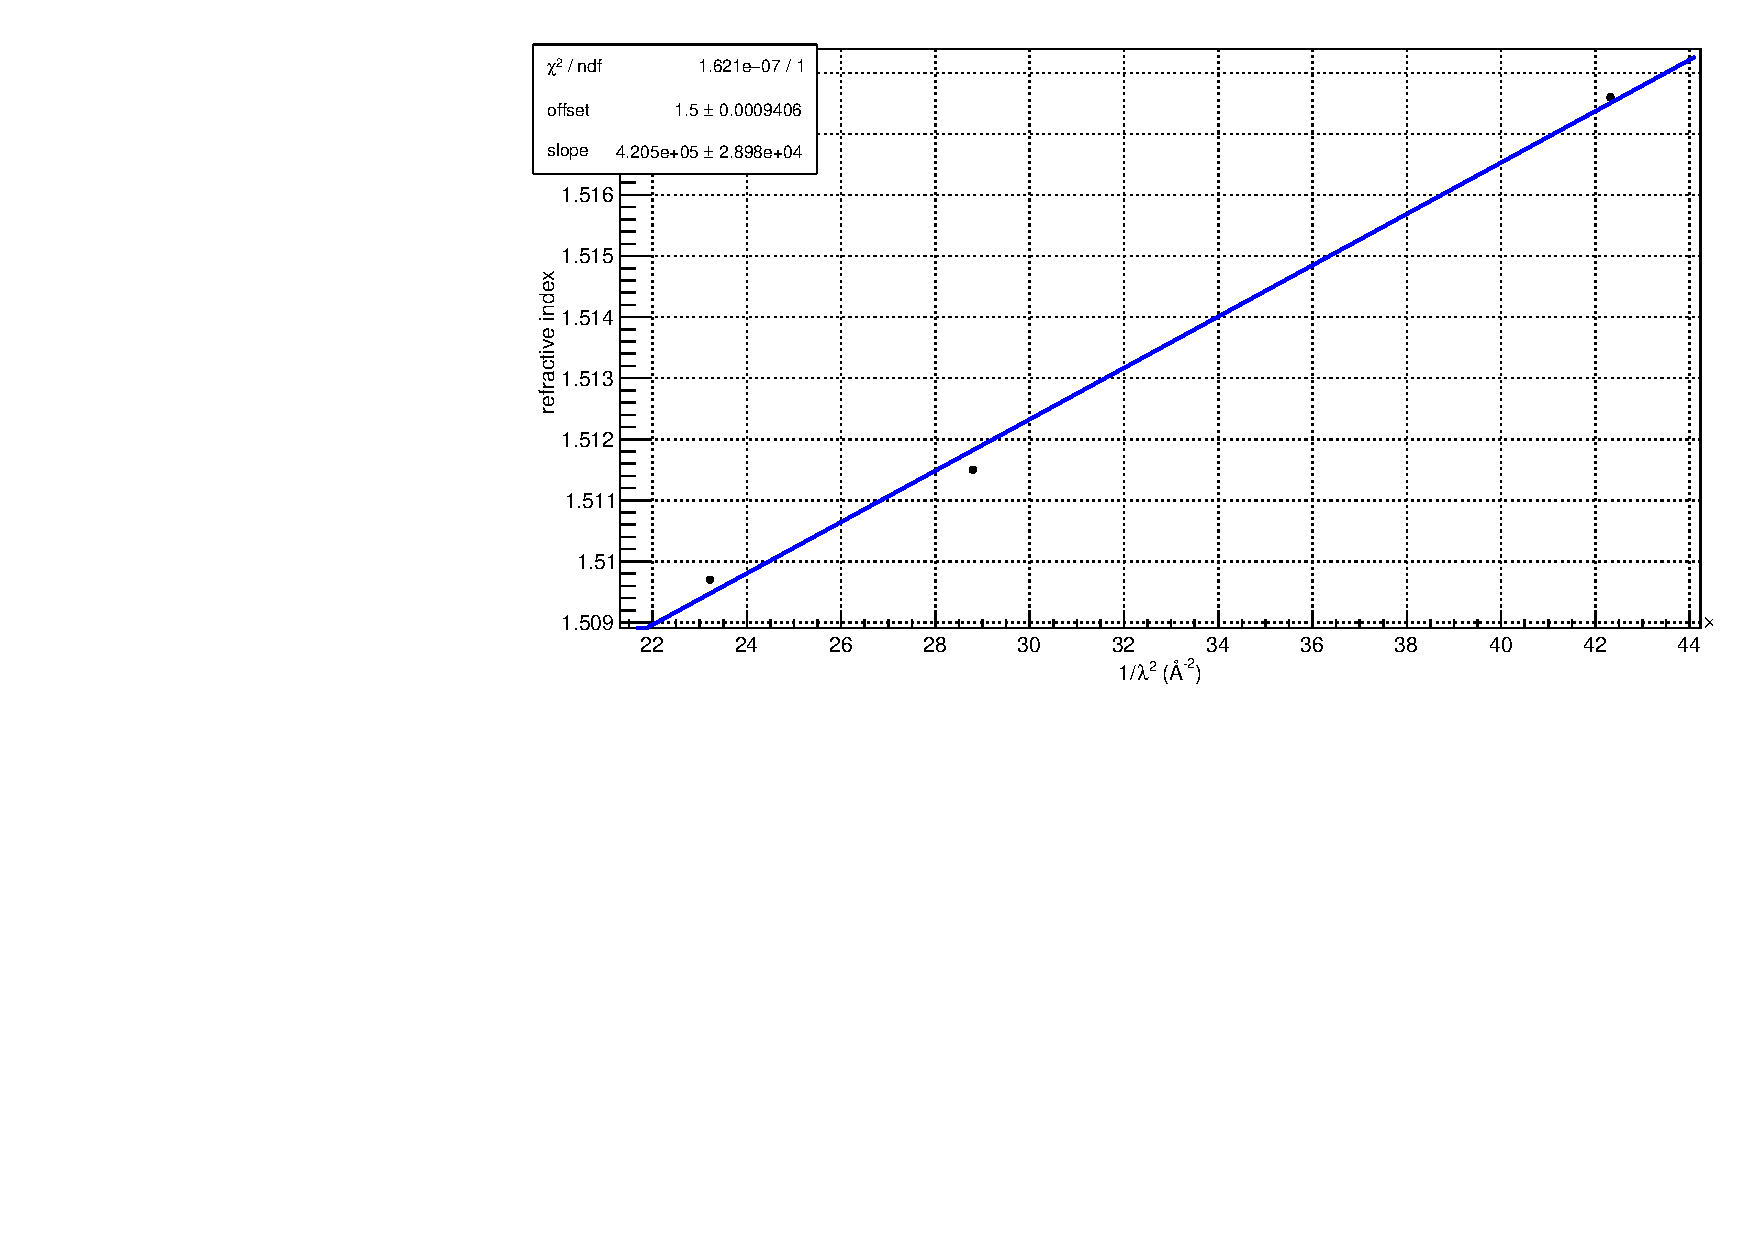
\includegraphics[scale=0.28, angle=0]{nFit}
%\caption{ Indice di rifrazione }
%\label{fig:alimentazione}
%\end{figure}
%\end{center}

Ottenendo quindi per $\lambda= 585.3 nm$ l'indice di rifrazione $n(\lambda)= 1.5119 \pm  $

\section*{Aquisizione ed analisi dati}
\paragraph{calibrazione}
Prima di procedere con la presa dati si è eseguita una calibrazione dell'apparato; in particolare è stato necessario regolare la posizione della sorgente rispetto all'apertura della fenditura.
Il primo passaggio è stato quindi impostare l'apertura della fenditura a $24 \mu m$ ed aquisire un primo spettro, zoomando sui primi 3/4 picchi dello spettro.
Successivamente si regola la posizione della sorgente cercando quella che massimizzi l'intensità della luce.
Si è quindi fissata la posizione: 0.93 mm.
Per regolare invece la larghezza dei picchi si è impostato l'apertura della fenditura a $18 \mu m$.
Infine si sono regolate le posizioni della lente focale e della lente condensante, scegliendo come posizioni ottimali rispettivamente 15.36 mm e 14.62 mm.


\subsection*{Campo magnetico spento}

Si quindi procede con l'acquisizione del primo spettro a campo magnetico spento: dopo aver selezionato il picco di interesse si inserisce la lamina di Lummer-Gerhcker, si seleziona quindi con i cursori il range dello scanning e si ruota la posizione del CCD in verticale.
Infine si imposta il tempo di integrazione a 600 ms e si avvia lo scanning, dopo aver salvato il file nell'opportuna cartella.

\paragraph{analisi dello spettro}



\section*{Conclusioni}



\newpage
\appendix
\section{Appendici}
\label{appendice}
\subsection{Costruzione dell'errore sulle misure}
\label{Calcerr}

\subsection{Tabella delle compatibilità}
\medskip
\begin{table}[H]
    \centering
    \begin{tabular}{c}
        %\hline
        \begin{Large}
        $\lambda=\frac{|a-b|}{\sqrt{\sigma_a^2+\sigma_b^2}}$
        \end{Large}\\
        %\hline
    \end{tabular}
    \hspace{0.5cm}
    \begin{tabular}{cc}
        \toprule
        &       \textbf{Compatibilità   }       \\
        \midrule
        0$\leq \lambda$<1   &Ottima                 \\
        1$\leq \lambda$<2   &Buona                  \\
        2$\leq \lambda$<3   &Accettabile            \\
        3$\leq\lambda$<5   &Pessima                \\
        $ \lambda \geq $  5     &Non compatibile        \\
        \bottomrule
    \end{tabular}
    \caption{indicazioni lettura compatibilità}
    \label{tab:compatibilità}
\end{table}

\subsection{Dati sperimentali}


   
\end{document}